\documentclass[11pt,oneside]{uhthesis}
\usepackage{subfigure}
\usepackage[linesnumbered,lined,titlenumbered,ruled]{algorithm2e}
\usepackage{amsmath}
\usepackage{amssymb}
\usepackage{amsbsy}
\usepackage{mathpazo}
\usepackage{float}
\usepackage{braket}
\setlength{\marginparwidth}{3cm}
\usepackage{todonotes}
\usepackage{mathtools} 
\usepackage[spanish]{babel}
\usepackage{graphicx}

\usepackage{listings}
\usepackage{color}
\usepackage{booktabs}
\usepackage{multirow}
\usepackage{ragged2e}
\newtheorem{defn}{Definición}
\floatstyle{ruled}
\restylefloat{table}
\usepackage{listings}
\usepackage{color}

\definecolor{dkgreen}{rgb}{0,0.6,0}
\definecolor{gray}{rgb}{0.2,0,0}
\definecolor{mauve}{rgb}{0.58,0,0.82}

\lstset{language=Lisp,
	aboveskip=10mm,
	belowskip=10mm,
	showstringspaces=false,
	columns=flexible,
	basicstyle={\small\ttfamily},
	keywordstyle=\color{blue},
	commentstyle=\color{dkgreen},
	stringstyle=\color{mauve},
	breaklines=true,
	breakatwhitespace=true,
	tabsize=3,
	numbers=left, numberstyle=\tiny, stepnumber=1,firstnumber=1,
	numbersep=5pt
}

\renewcommand{\tablename}{Tabla}
\title{Proceso de Evaluación Automática en Problemas de Enrutamiento de Vehículos}
\author{Josué Rodríguez Ramírez}
\advisor{MSc. Fernando Rodríguez Flores}
\coadvisor{Lic. Rodrigo García Gómez}
\degree{Licenciado en Ciencias de la Computación}
\faculty{Facultad de Matemática y Computación}
\date{Noviembre de 2023}
\logo{Graphics/uhlogo}

\renewcommand{\vec}[1]{\boldsymbol{#1}}
\newcommand{\diff}[1]{\ensuremath{\mathrm{d}#1}}

\begin{document}
\selectlanguage{spanish}
\maketitle

%\frontmatter
\include{FrontMatter/Dedication}
\begin{acknowledgements}

    Le agradezco a Dios, en primer lugar, por escogerme y darme la oportunidad de estudiar esta carrera.

    A mi tutor Fernando y mi cotutor Rodrigo por dedicarme parte de su tiempo para desarrollar este trabajo y por su paciencia inagotable.

    Agradezco a mis padres y pastores que me han aconsejado, alentado y nunca se cansaron de orar por mí. Al resto de mi familia que me motivaron para llegar hasta aquí.
    
    A mis hermanos en la fe, que oraron incensantemente por esta tesis.

\end{acknowledgements}

\begin{opinion}	

La tesis de Josué presenta una metodología para resolver distintas variantes del VRP con poco tiempo de trabajo humano, aprovechando Algoritmos de Búsqueda Local. Lo más notable es que su enfoque elimina la necesidad de programar manualmente la evaluación de soluciones vecinas de casi cualquier variante, ya que este proceso se automatiza de manera eficiente en su propuesta. Este avance representa un paso importante en la optimización de recursos y tiempo en la investigación relacionada con el VRP.

Josué ha demostrado su capacidad para aplicar de manera creativa los conocimientos adquiridos durante su carrera. Ha demostrado una habilidad notable para identificar y resolver problemas emergentes en su investigación, destacándose en la adquisición autodidacta de conocimientos y habilidades necesarias para este proyecto. Su enfoque innovador ha sido fundamental en el éxito de su trabajo.

Estamos convencidos de que la tesis de Josué es un claro testimonio de su aptitud para desempeñarse como un destacado Científico de la Computación. Su investigación cumple con todos los requisitos de una tesis de licenciatura en este campo y pone de manifiesto su potencial para contribuir a la ciencia el futuro. Estamos seguros de que Josué continuará avanzando y enriqueciendo esta disciplina con sus futuras contribuciones.

\vspace{1cm}


\begin{flushright}
	\underline{\hspace{6.5cm}}\\
	MSc. Fernando Raúl Rodríguez Flores
	
	Facultad de Matemática y Computación
	
	Universidad de la Habana
	
	Noviembre, 2023
\end{flushright}

\end{opinion}
\begin{abstract}
En este trabajo se presenta un método que evalúa de manera automática las soluciones vecinas de cualquier Problema de Enrutamiento de Vehículos (VRP). La estructura que se propone permite corregir deficiencias del Grafo de Evaluación desarrollado en otra tesis de licenciatura. A esta propuesta se le aplica una cinta computacional basada en la idea que se utiliza en la Diferenciación Automática. Las soluciones vecinas podrán evaluarse sin tener que implementar un código específico para ello y el uso de la cinta garantiza que se evalúen solo las partes de la solución inicial que se modificaron para obtener la nueva solución. Esta propuesta es extensible para cualquier variante de VRP, solo se necesita el código de evaluación de la primera solución.
\end{abstract}

\begin{enabstract}
In this work, a method that automatically evaluates the neighboring solutions of any Vehicle Routing Problem (VRP) is presented. The proposed structure makes it possible to correct deficiencies in the Evaluation Graph developed in another bachelor's thesis. To this proposal a computational tape is applied based on the idea that Automatic Differentiation is used. Neighboring solutions can be evaluated without having to implement specific code for this, and the use of the tape ensures that only those parts of the initial solution that were modified to obtain the new solution are evaluated. This proposal is extensible for any VRP variant, only the evaluation code of the first solution is needed.
\end{enabstract}
\include{FrontMatter/Contents}

%\mainmatter
\chapter*{Introducción}\label{chapter:introduction}
\addcontentsline{toc}{chapter}{Introducción}

\qquad 
Los Problemas de Enrutamiento de Vehículos (VRP~por sus siglas en inglés) son problemas logísticos en los que las empresas invierten hasta el 20\% de sus ganancias \cite{Toth}. Una optimización de las estrategias de solución de estos problemas significaría un ahorro significativo del presupuesto destinado a resolverlos. 

Los VRP son un grupo de problemas de optimización combinatoria que tienen como objetivo determinar un conjunto de rutas para una flota de vehículos que parten de uno o más depósitos para satisfacer las demandas de un grupo de clientes distribuidos en una zona determinada. A su vez, se desea optimizar el costo de algún recurso, ya sea capacidad, combustible, tiempo \cite{Hillier}.

El problema original se modifica en dependencia de las demandas de los clientes y a partir de estas modificaciones surgen múltiples variantes como: 
\begin{itemize}
	\item VRP con recogida y entrega (VRPPD) que tiene el objetivo de encontrar una serie de rutas para un conjunto de vehículos que deben suministrar servicio a clientes, con la restricción de que los vehículos tengan suficiente capacidad de transporte para los productos (o personas) que deben ser recogidos y/o entregados a cada cliente (nodo) \cite{PedroP},

    \item VRP con ventanas de tiempo (VRPTW) donde una flota fija de vehículos de capacidad limitada está disponible en un depósito para atender a un conjunto de clientes con demandas determinadas y cada cliente debe ser visitado dentro de un período de tiempo determinado \cite{Kolen}, 
	\item VRP con más de un depósito (MDVRP) \cite{Bayir, Alemany}, 
	\item VRP con restricciones de capacidad (CVRP) donde cada vehículo tiene una capacidad limitada \cite{Alemany}, por solo mencionar algunas. 
\end{itemize}
	Cada una de ellas presenta características que la diferencian del resto, por lo que resulta difícil plantear un método genérico que resuelva cualquier VRP\@.

Estos problemas son NP-duros \cite{Garey}, que son los problemas que no se pueden resolver en un tiempo polinomial. El tiempo y esfuerzo computacional requerido para resolver los VRP aumenta exponencialmente respecto al tamaño del problema. Por esta razón, se deben resolver con métodos aproximados como las heurísticas o metaheurísticas.

Algunos de estos algoritmos son basados en poblaciones como los algoritmos genéticos \cite{Mester}, otros como SA (Simulated Annealing) \cite{Liu}, LNS (Large Neighborhood Search) \cite{Ropke} y VNS (Variable Neighborhood Search) \cite{Camila} que se basan en una búsqueda local.

Para solucionar un VRP mediante un algoritmo de búsqueda local se parte de una solución inicial $S_{0}$ a la que se le hacen transformaciones, como cambiar de rutas, vehículos o clientes y, a partir de estos cambios se obtiene un conjunto de nuevas soluciones que se denomina vecindad de $S_{0}$. De este conjunto se selecciona una solución $S_{1}$ y a partir de esta última se repite el proceso hasta que se cumpla algún criterio de parada \cite{JJ}. 

El problema a resolver es que para evaluar cada una de las nuevas soluciones se debe programar un algoritmo de evaluación, que es diferente en cada VRP. ¿Cómo se puede automatizar el proceso de evaluación de todas las soluciones? ¿Cómo generalizar ese proceso para todos los Problemas de Enrutamiento de Vehículos?

En este trabajo se plantea un método para calcular el costo de las nuevas soluciones para cualquier problema de enrutamiento de vehículos de manera automática. Esto se realiza a través de una estructura denominada \textit{cinta computacional}, es decir, una lista de las transformaciones que se apliquen a la solución inicial.

Esta misma estructura se utiliza en el proceso de diferenciación automática que calcula las derivadas de una función matemática de manera exacta y con la mayor precisión posible en un tiempo razonable que en la mayor parte de los casos prácticos no excede de un pequeño múltiplo del propio tiempo de evaluación de la función \cite{Manuel,Griewank}.

En la Facultad de Matemática y Computación de la Universidad de La Habana se desarrollan métodos de solución generalizados para todas las variante de VRP. Por ejemplo, en \cite{Camila} se desarrolla una metaheurística de Búsqueda Local (IVNS, por sus siglas en inglés) que permite considerar infinitos criterios de vecindad para un problema, utilizando gramáticas libres del contexto. 

Por su parte, en \cite{JJ} se presenta una forma de calcular el costo de un vecino en casi cualquier variante de VRP, utilizando una estructura llamada Grafo de Evaluación. Algunas variantes, como el Problema de Enrutamiento de Vehículos con Entregas y Recogidas Simultáneas no son solucionadas con esta propuesta. La solución que se presenta en este trabajo resuelve todas las variantes de los VRP y extiende la investigación realizada por \cite{JJ}. 

\subsection*{Objetivos}
El objetivo de este trabajo es desarrollar una estructura que evalúe de manera autómatica las soluciones vecinas de cualquier problema de enrutamiento de vehículos, a partir del grafo de evaluación propuesto en \cite{JJ}. Para eso se implementa una cinta computacional basada en la idea de la diferenciación automática.

Para lograr los objetivos generales se han trazado los siguientes objetivos específicos:

\begin{enumerate}
	\item Consultar literatura especializada sobre el estado del arte de los problemas VRP.
	\item Estudiar las ideas y códigos relacionados con el Grafo de Evaluación \cite{JJ}
	\item Diseñar e implementar una cinta computacional a partir del Grafo de Evaluación.	
	\item Analizar los resultados obtenidos en diferentes variantes de VRP.
\end{enumerate}

El presente documento está organizado en 4 capítulos.

En el capítulo \ref{chapter: VRP} se describen las caraterísticas fundamentales de los problemas de enrutamiento de vehículos y los algoritmos de búsqueda local. En el capítulo \ref{chapter: AD} se describe la estrategia utilizada en la diferenciación automática y cómo aplicarla a los VRP. El capítulo \ref{chapter: Automatic-Eval} describe el proceso y la estructura implementados. En el capítulo \ref{chapter: Results} se exponen los resultados alcanzados. Se presentan, además, las conclusiones obtenidas a partir de este trabajo y se brindan algunas recomendaciones para la extensibilidad del sistema en trabajos futuros.






\chapter{Preliminares}\label{chapter: VRP}

En este trabajo se presenta el proceso de evaluación automática de las soluciones vecinas, que se obtienen en los algoritmos de búsqueda local, para cualquier VRP.

Este capítulo presenta los conceptos básicos de los problemas de enrutamiento de vehículos y los algoritmos de búsqueda local. Además, se definen los criterios de vecindad que se utilizan en el sistema y la estructura de datos que se utiliza para evaluar soluciones parciales de manera automática.

En la sección \ref{1-VRPintro} se presentan las características principales de los VRP. En la sección \ref{2-LocalSearch} se describen los algoritmos de búsqueda local. En la sección \ref{3-Criterias} se explican los criterios de vecindad que se utilizan en el sistema. En la sección \ref{3-EvalGraph} se describe el grafo de evaluación que se utiliza para evaluar las soluciones vecinas en cada VRP.

%\newpage

\section{Problema de Enrutamiento de Vehículos}\label{1-VRPintro}
Desde 1959, cuando George Dantzig y John Ramser introducen la primera definición de un VRP\cite{Dantzing}, se han desarrollado variantes asociadas a las demandas de los clientes del problema. Estas demandas pueden ser el tiempo de espera, la entrega y recogida de paquetes o la capacidad de los vehículos. 

Todos los VRP presentan uno o múltiples depósitos iniciales, de donde parten los vehículos para satisfacer las demandas de cada cliente. El recorrido termina en los depósitos.

A continuación, en \ref{fig:vrp-variants} se presentan esquemas de diferentes variantes de VRP. En la primera variante (CVRP) cada vehículo presenta una capacidad \cite{Alemany}. La segunda variante (VRPWT) muestra clientes con ventanas de tiempo \cite{Kolen}. En la tercera variante (MDVRP) se aprecia más de un depósito para la flota de vehículos \cite{Bayir, Alemany}. 


\begin{figure}
	\centering
	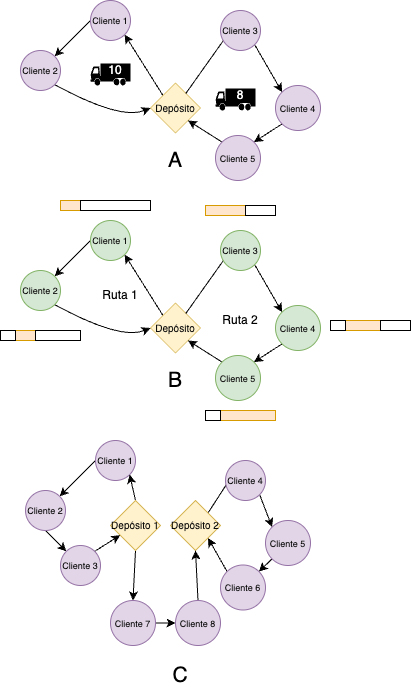
\includegraphics[width=0.7\linewidth]{Graphics/VRP}
	\caption{Variantes del VRP. A: CVRP. B: VRPTW. C: MDVRP.}
	\label{fig:vrp-variants}
\end{figure}

Como se puede notar, sería muy dificil encontrar un algortimo general que resuelva cualquier VRP, dado que estos problemas presentan restricciones diferentes y, por lo tanto, estrategias diferentes para solucionarlos. Estas estrategias son heurísticas o metaheurísticas que se adaptan a las características específicas de un tipo específico de VRP. En la siguiente sección se presenta la búsqueda local, en la que se basan un grupo de estas metaheurísticas.

%Soluciones con la búsqueda local

\section{Algoritmos de Búsqueda Local}\label{2-LocalSearch}

En los algoritmos de búsqueda local se parte de una solución inicial $S_{0}$, que se modifica de varias maneras para obtener un conjunto $NS_{0}$ llamado conjunto de soluciones vecinas de $S_{0}$, o vecindad de $S_{0}$\cite{JJ}. A las reglas que se aplican para modificar una solución y obtener las soluciones vecinas se les conoce con el nombre de estructura de entorno o criterio de vecindad\cite{JJ}. Del conjunto de soluciones $NS_{0}$ se extrae una nueva solución a modificar. Esto se realiza hasta cumplir con algún criterio de parada.

Existen diferentes algoritmos que se basan en la búsqueda local. Por ejemplo, \textit{Simulated Annealing}\cite{Liu}, \textit{Tabu Search}\cite{Taillard1997}, \textit{Variable Neighborhood Search}\cite{Camila}. Estos algoritmos difieren en los criterios utilizados para obtener las soluciones vecinas. La siguiente sección trata sobre esos criterios de vecindad.

%Criterios de vecindad
\section{Criterios de vecindad}\label{3-Criterias}

Los criterios de vecindad son reglas para transformar una solución de un problema determinado y obtener nuevas soluciones. Para el caso de VRP, estos criterios pueden ser \textit{``cambiar un cliente de posición''}, \textit{''intercambiar dos clientes''}, o \textit{''cambiar el vehículo de una ruta''}.

Estos criterios se pueden describir como una secuencia de operaciones elementales. Algunas de estas pueden ser:

\begin{enumerate}
	\item Seleccionar una ruta \texttt{r}. 
	\item seleccionar un cliente \texttt{c} de una posición \texttt{p} de una ruta \texttt{r}.
	\item insertar un cliente \texttt{c} en una posición \texttt{p} de una ruta \texttt{r}.
\end{enumerate}

Por ejemplo, el criterio \textit{cambiar un cliente de posición} está compuesto por las operaciones \textit{extraer cliente de una posición dada} e \textit{insertar al cliente en otra posición},
mientras que el criterio \textit{cambiar el vehículo de una ruta} puede componerse por las operaciones \textit{ extraer vehículo de ruta} y \textit{ asignar a una ruta dada un determinado vehículo disponible}.

Los criterios de vecindad utilizados en un algoritmo de búsqueda local dependen de la variante de VRP que se esté resolviendo \cite{Daniela}. Por ejemplo, en un problema donde la flota de vehículos es homogénea pero existen varios depósitos, la operación \textit{cambiar vehículo} no tiene sentido pero \textit{cambiar depósito} sí puede aplicarse.

Para evaluar cada una de las soluciones vecinas del VRP y aplicar los criterios de vecindad, se utiliza una estructura de datos llamada grafo de evaluación que se define en la siguiente sección. Este grafo se usa para evaluar de manera automática la solución del problema, es decir, sin que sea necesario escribir el código de la evaluación.

% Grafo de Evaluación
\section{Grafo de Evaluación}\label{3-EvalGraph}

A partir de la solución inicial del VRP se crea un grafo que se utilizará para evaluar las soluciones vecinas obtenidas por los criterios de vecindad en cada problema del VRP.

En \cite{JJ} se define formalmente la estructura del grafo de evaluación.

\begin{defn}
	Entidad del problema: Cada uno de los elementos que componen la solución de una determinada variante de un VRP.
\end{defn}
  
  Por ejemplo, en un problema con flota heterogénea las entidades del problema serían los clientes, los vehículos y el depósito central. En este trabajo se presentan como \textit{variables iniciales}.
  
  \begin{defn}
	  Información del problema: Dato que forma parte de la entrada del problema.
  \end{defn}
  
  Un ejemplo de información en el CVRP es la demanda de cada cliente y también la distancia entre cada par de clientes. Para el HFVRP, la capacidad
  de cada vehículo es también una información del problema.
  
  \begin{defn}
	Variable: Se refiere a toda variable que se use durante la evaluación de una solución y contenga un valor numérico que no sea información del problema ni entidad del problema.
  \end{defn}
  Ejemplos de variables serían \textit{distancia-total, demanda-de-ruta, }etc. En este trabajo se presentan como variables intermedias.


  \begin{defn}
	  Operación: Función que se aplica durante la evaluación de una solución.
  \end{defn}
  
  Durante la evaluación de una determinada solución es común aplicar operaciones entre las variables como \textit{incrementar distancia total, aumentar o disminuir la carga de un vehículo, penalizar exceso de carga,
  }etc.
  
  \begin{defn} \label{def:op-node}
	  Nodo operacional: Nodo que representa una operación.
  \end{defn}
  
  Un nodo operacional es la representación en el grafo de evaluación de una operación. Toda operación recibe una entrada y
  provoca que se transforme  una determinada salida. Por ejemplo, cuando se aplica la operación \textit{incrementa la distancia total en la distancia entre los clientes 1 y 2}
  se incrementa el valor contenido en la variable \textit{distancia-total} (salida) en dependencia de la distancia entre los clientes 1 y 2 (entradas).
  
 En este trabajo, los nodos operacionales son parte de las variables intermedias, y se les asocia la operación. También se le asocia dos métodos, el método de evaluación, que se utiliza para evaluar las demandas de las variables, y el método de desevaluación, que vuelve atrás la evaluación realizada; es decir hace la operación inversa de la evaluación.

  En la definición \ref{def:op-node} se establece la representación de una operación, por tanto se hace necesario definir la representación de las entradas y las salidas de dichas
  operaciones.
  
  \begin{defn}
	  Nodo de entrada/salida: Nodo que representa la entrada o la salida de alguna operación.
  \end{defn}
\subsection*{Construcción del grafo de evaluación}
Para construir este grafo, en primer lugar, se realiza un proceso de inicialización, donde se construyen únicamente los nodos principales de dicho grafo, que son los correspondientes a cada cliente y depósito. A continuación se muestra un ejemplo del grafo inicializado.

En el ejemplo se presentan 4 clientes (1,2,3,4) y dos rutas (A,B). Un vehículo comienza en un depósito y recorre a los clientes 1, 2 y 3 que se encuentran en A y regresa al depósito, otro vehículo visita al cliente 4 que pertenece a la ruta B:
\begin{displaymath}
A = [1,2,3]          B = [4]
\end{displaymath}
En la figura \ref{fig:vrp-initialGraph} se muestra cómo se inicializa el grafo.

\begin{figure}[htb]
	\centering
	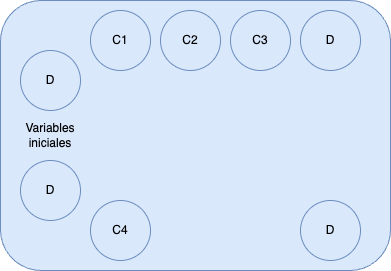
\includegraphics[width=0.7\linewidth]{Graphics/Init}
	\caption{Grafo inicializado.}
	\label{fig:vrp-initialGraph}
\end{figure}

Un grafo inicializado no contiene ninguna arista debido a que en un grafo de evaluación las aristas indican las entradas y las salidas de las operaciones que se realizan en la evaluación de la solución\cite{JJ}.

Luego de inicializado el grafo se desarrollan los nodos intermedios a partir del código de evaluación de la solución inicial. En la figura se presenta el código que evalúa una solución del VRP. La operación \texttt{d(x,y)} representa la distancia entre \texttt{x} e \texttt{y}.

\begin{lstlisting}
evaluate(S):
  new_var total_distance = 0
  for each route r in S:         
      new_var route_demand = 0
      new_var prev_client = depot(r)
      for each client c in r:
          increase total_distance with d(prev_client, c)
          increase route_demand with demand of client c
          prev_client = c
      increase total_distance with d(c, depot) 
      increase total_distance with penalize(demand_route, vehicle_capacity)
   return total_distance        
\end{lstlisting}

En ese proceso de evaluación se realizan operaciones para obtener el costo de la solución. Estos costos pueden ser la distancia recorrida, la demanda de la ruta, la penalización de la ruta, etc. Para guardar el resultado de estas operaciones se crean nuevos nodos, que llamaremos nodos intermedios.

A continuación se muestra el grafo de evaluación de la primera solución del VRP.

En la figura \ref{fig:vrp-Graph-process1} se muestra la creación de una variable intermedia asociada al cliente 1 para guardar el costo de la ruta del depósito al cliente 1. Además, se crea un nodo para guardar la penalización de la ruta y un nodo para guardar la suma total de la ruta 1.

\begin{figure}[htb]
	\centering
	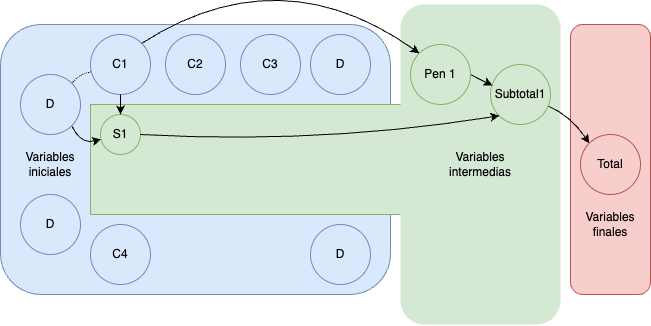
\includegraphics[width=0.7\linewidth]{Graphics/Graph-process}
	\caption{ Proceso del grafo de evaluación comenzando con el cliente 1.}
	\label{fig:vrp-Graph-process1}
\end{figure}

En la figura \ref{fig:vrp-Graph-process2} se muestra que la evaluación de la ruta 1 está calculada.

\begin{figure}[htb]
	\centering
	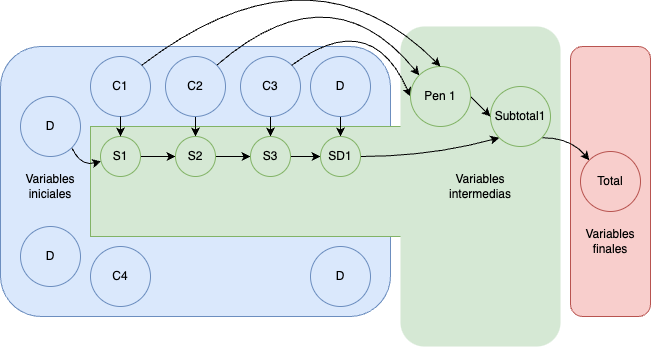
\includegraphics[width=0.7\linewidth]{Graphics/Graph-process2}
	\caption{Proceso del grafo de evaluación a terminar la ruta A.}
	\label{fig:vrp-Graph-process2}
\end{figure}

Por último, en la figura \ref{fig:vrp-Graph-process3} se presenta el grafo de evaluación para esta solución.

\begin{figure}[htb]
	\centering
	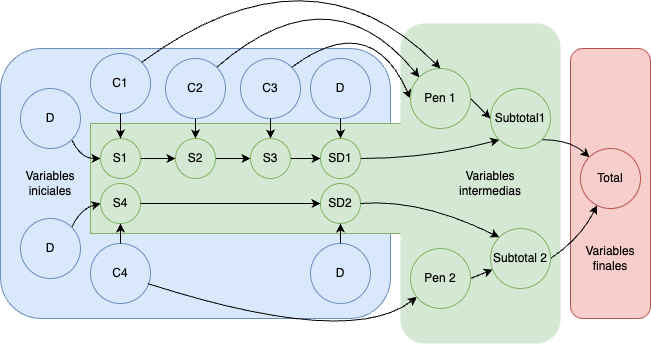
\includegraphics[width=0.7\linewidth]{Graphics/Graph-process3}
	\caption{Proceso del grafo de evaluación terminado.}
	\label{fig:vrp-Graph-process3}
\end{figure}

Se puede comprobar que el grafo ha guardado cada cálculo parcial de la evaluación de la solución en las variables intermedias creadas, de tal manera que, al aplicar un criterio de vecindad a la solución puede evaluarse sin necesidad de hacer el proceso de evaluación completo nuevamente. Si a la solución anterior se aplicara, por ejemplo, la operación eliminar cliente C3 como se muestra en la figura  \ref{fig:vrp-deleteClient} entonces no se modifica el valor del cálculo que se realizó antes de visitar este cliente o el valor calculado de otra ruta. 

La soluciones, que se obtienen cuando se aplica un criterio de vecidad a la solución anterior, pueden evaluarse de manera automática a partir de la solución previa, sin necesidad de escribir un nuevo código de evaluación. En el ejemplo \ref{fig:vrp-deleteClient} se pasa de la suma parcial del cliente 2 a la suma parcial del depósito.

\begin{figure}[htb]
	\centering
	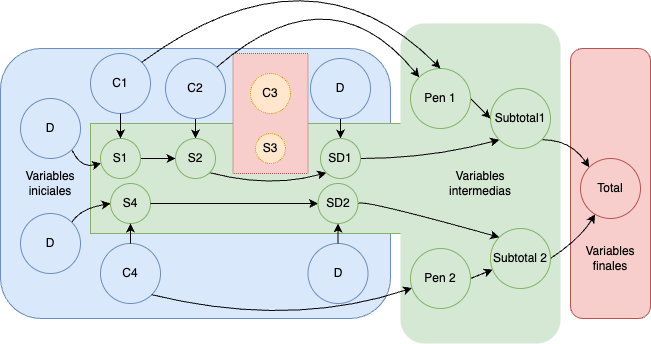
\includegraphics[width=0.7\linewidth]{Graphics/DeleteClient}
	\caption{Grafo de evaluación transformado al eliminar el cliente 3.}
	\label{fig:vrp-deleteClient}
\end{figure}

Otro ejemplo sería eliminar este cliente C3 en la ruta A e insertarlo en la ruta B como se presenta en la figura \ref{fig:vrp-changeClient}. En este caso, en la ruta A se evalúa sólo a partir de la suma parcial 2 como en el ejemplo anterior, ya que no se modifica el valor calculado previamente. Además, debe evaluarse la ruta B a partir del cliente insertado porque el valor calculado de la ruta hasta el cliente anterior no se modificó.

\begin{figure}[htb]
	\centering
	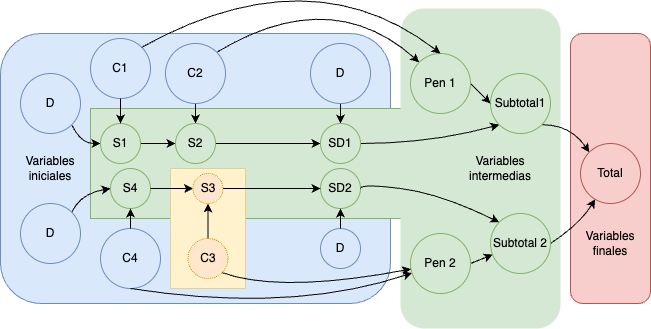
\includegraphics[width=0.7\linewidth]{Graphics/ChangeClient}
	\caption{Grafo de evaluación transformado al cambiar el cliente 3 de la ruta A a la ruta B.}
	\label{fig:vrp-changeClient}
\end{figure}

Los nodos intermedios hacen función de variables acumuladoras, porque guardan el costo de cumplir la demanda de cada cliente y las aristas describen el siguiente nodo a evaluar que depende del valor de nodo anterior.

El proceso de calcular a partir de un nodo o evaluar la ruta desde el depósito hasta el nodo final, depende de una cinta computacional que se conecta a este grafo de evaluación. La idea de esta cinta surge de la Diferenciación Automática que se explica en el siguiente capítulo.
% Chapter 2 Cinta de la Diferenciación automática

% Chapter 3 Mezcla y código en Lisp

% Chapter 4 Resultados

% Conclusiones, recomendaciones y bibliografía





























\chapter{Diferenciación Automática}\label{chapter: AD}

Para obtener la estructura automática que evalúe cada variante de VRP, así como los problemas vecinos, que se obtienen cuando se aplican los criterios de vecindad, sin necesidad de reestructurar el código, se utiliza una cinta computacional. Esta cinta se aplica, de manera similar, en el proceso matemático de Diferenciación Automática (AD, por sus siglas en inglés) y se explica en este capítulo.

Este capítulo está dividido en 5 secciones. La sección \ref{2:AD-process} trata sobre el concepto de diferenciación automática. La sección \ref{2:eval-modes} presenta y describe los dos modos de evaluación de esta estrategia. La sección \ref{2:tape} presenta la estructura de la cinta de evaluación que utiliza AD.
\section{Proceso de Diferenciación Automática (AD)}\label{2:AD-process}
En esta sección se presenta el concepto y las caraterísticas de la Diferenciación Automática.

AD es una estrategia que se utiliza para evaluar la derivada de una función matemática a través de un código computacional. Se utiliza la regla de la cadena y se obtiene la evaluación de las derivadas sin errores numéricos.

La información durante el proceso de evaluación se guarda en variables intermedias, dentro de una cinta de evaluación, que no es más que el registro de una corrida en particular de un programa dado, con valores particulares especificados para las variables de entrada, mostrando la secuencia de valores intermedios calculados y las operaciones realizadas. A esta cinta de evaluación también se le conoce con el nombre de \textbf{procedimiento de evaluación}. En caso de una reestructuración de la función inicial, se mantendrá guardada la información de las partes no alteradas de la función. Estas partes no modificadas de la función no se vuelven a evaluar y de esta manera no se repiten cálculos innecesarios. A continuación se muestra un ejemplo de cómo se usa esta estrategia de evaluación:

Sea la función $y = f(x1,x2)$ donde:
\begin{equation}
	\label{eq:example}
y = tan(x1) * \frac{x1}{x2} + sen(x2) * cos(x1)
\end{equation}

Se quiere calcular el valor de $y$ en algún punto $(x_{1}^{*},x_{2}^{*})$.
El Cuadro \ref{tab:table1} muestra la manera en la que se evalúa la función aplicando esta estrategia de evaluación automática. Se muestra una secuencia de variables, las primeras son variables de entrada; luego siguen las intermedias (denotadas por $V_{i}$ con $i>0$),y al final las de salida (en este caso es $y$). Cada variable es calculada a partir de aquellas definidas previamente aplicando una de las operaciones o funciones elementales: suma, resta, multiplicación, seno, exp, etc.

El procedimiento de evaluación no se corresponde directamente con la expresión de $f$ como fue escrita originalmente, sino con una expresión cuya evaluación es más eficiente mediante sub-expresiones repetidas, evaluadas una vez, y luego reutilizadas. El procedimiento de evaluación captura la secuencia precisa de operaciones y argumentos usados por una implementación particular de un algoritmo o función. Las expresiones generadas serán reutilizadas para la evaluación de las derivadas.

\begin{table}[h]
\begin{center}
\begin{tabular}{|l|} \hline
			$\begin{aligned}
			v_{-1} & = x_{1}	   \\
			v_{0}  & = x_{2}\\
			\end{aligned}$   	
			\\ \hline
			
			$\begin{aligned}
			\ \ v_{1} & = tan(v_{-1})   \\
			\ \ v_{2} & = v_{-1}/v_{0}  \\
			\ \ v_{3} & = v_{1}*v_{2}   \\
			\ \ v_{4} & = sen(v_{0})   \\
			\ \ v_{5} & = cos(v_{-1}) \\
			\ \ v_{6} & = v_{4}*v_{5} \\
			\ \ v_{7} & = v_{3}+v_{6}\\
			\end{aligned}$
			\\ \hline
			$\begin{aligned}
			\ \ \ y &= v_{7} 
			\end{aligned}$
			\\ \hline
\end{tabular}
		\caption{Cinta para la evaluación de la función del ejemplo \ref{eq:example}}
		\label{tab:table1}
\end{center}
\end{table}

Este procedimiento utiliza un grafo computacional que se presenta en la siguiente sección.

\section{Grafo computacional}\label{2:graph}
La relación entre las variables, es decir, las dependientes e independientes se presentan en un grafo computacional, parecido al utilizado en el sistema de VRP. Para el ejemplo mostrado en esta sección aquí se tiene la Figura \ref{fig:ADgraph}.

\begin{figure}[htb]
	\centering
	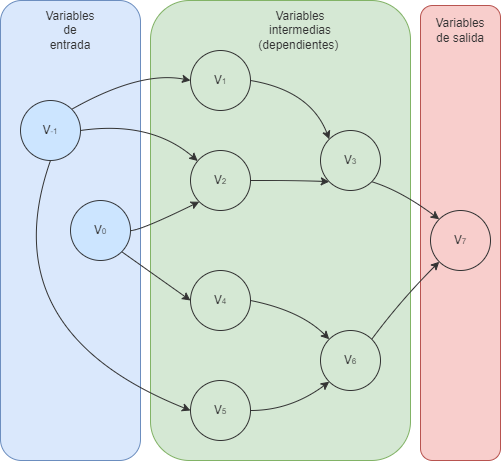
\includegraphics[width=0.5\linewidth]{Graphics/ADgraph}
	\caption{Grafo de evaluación para el ejemplo, se distinguen los diferentes tipos de variables.}.\label{fig:ADgraph}
\end{figure}
		
Como se puede notar las raíces del grafo son las variables independientes mientras que los demás nodos son variables dependientes. La diferenciación automática utiliza dos maneras básicas de propagar las derivadas a través de la cinta y así llevar la información precalculada a los siguientes niveles para su uso. Uno es el modo \textit{forward} y el otro el modo \textit{reverse} que serán tratados en la siguinte sección.

\section{Modos de evaluación}\label{2:eval-modes}

El modo forward o hacia adelante consiste en propagar derivadas desde variables independientes o de entrada, y a través de variables intermedias hasta variables dependientes o de salida del programa, siguiendo el flujo de ejecución del mismo.

De forma general, se aplica la regla de la cadena para cada variable intermedia $v_{i}$ que se calcula, almacenando los valores obtenidos en nuevas variables $v^{*}_{i}$, que a la vez se utilizan en las subsiguientes aplicaciones de la regla de la cadena a lo largo de la ejecución del programa, hasta propagar las derivadas a las variables dependientes.

Para mostrar cómo funciona el modo forward se toma el ejemplo \ref{eq:example}. El resultado se muestra en el cuadro \ref{tab:table2}.

Cada $v_{i}$ representa las variables vistas en el Cuadro \ref{tab:table1} y cada $v_{i}^{*}$ representa su derivada que será propagada.

\begin{table}[htp]
		\begin{center}
			\begin{tabular}{|l|} \hline
			$\begin{aligned}
			
			v_{-1}&=x_{1}     \\
			v_{-1}^{*}&=x_{1}^{*}	   \\
			v_{0}&=x_{2} 	   \\ 
			v_{0}^{*}&=x_{2}^{*}
			\end{aligned}$
			\\ \hline
			$\begin{aligned}
			\ \ v_{1}&=tan(v_{-1})   \\
			v_{1}^{*}&=1/cos^{2}(v_{-1})*v_{-1}^{*} \\
			v_{2}&=v_{-1}/v_{0}  \\
			v_{2}^{*}&=(v_{-1}^{*}*v_{0}-v_{0}^{*}*v_{-1})/v_{0}^{2} \\
			v_{3}&=v_{1}*v_{2}   \\
			v_{3}^{*}&=v_{1}^{*}*v_{2}+v_{2}^{*}*v_{1} \\
			v_{4}&=sen(v_{0})   \\
			v_{4}^{*}&=cos(v_{0})*v_{0}^{*}   \\
			v_{5}&=cos(v_{-1}) \\
			v_{5}^{*}&=-sen(v_{-1})*v_{-1}^{*} \\
			v_{6}&=v_{4}*v_{5} \\
			v_{6}^{*}&=v_{4}^{*}*v_{5}+v_{5}^{*}*v_{4} \\
			v_{7}&=v_{3}+v_{6} \\
			v_{7}^{*}&=v_{3}^{*}+v_{6}^{*} \\
			\end{aligned}$	
			\\ \hline
			$\begin{aligned}
			\ \ y = v_{7} \\
			\ \ y^{*} = v_{7}^{*} \\
			\end{aligned}$		
			\\ \hline
			\end{tabular}
		\caption {Procedimiento de evaluación de la derivada con el modo forward.} 
		\label{tab:table2}
		\end{center}
\end{table}

De la tabla \ref{tab:table1} a la \ref{tab:table2} se realiza un procedimiento completamente mecánico. Cada expresión original es sucedida por una correspondiente expresión derivada, de manera que la longitud del procedimiento de evaluación derivado es el doble del original.

El modo reverse o hacia atrás, una vez ejecutado el procedimiento de evaluación de la función hacia adelante, la información de las derivadas se propaga en sentido contrario al flujo de ejecución del programa, desde las variables dependientes o de salida, y a través de las variables intermedias hasta las variables independientes o de entrada.

De forma general, por cada variable intermedia $v_{i}$ se genera una variable llamada \textit{variable adjunta} $v^{*}_{i}$, que acumula incrementalmente los valores $v^{*}_{i}* \frac{\partial{y_{j}}}{\partial{v_{i}}}$ para todas las variables $v_{j}$ que dependen de $v_{i}$ donde $y_{j}$ es una función que describe precisamente esa dependencia.

A continuación se muestra el resultado de aplicar el modo reverse al ejemplo \ref{eq:example}. La fase hacia adelante es la misma que en el Cuadro \ref{tab:table1}. El resultado de la fase hacia atrás se muestra en el cuadro \ref{tab:table3}.

\begin{table}[htp]
	\begin{center}
		\begin{tabular}{|l|} \hline
			$\begin{aligned}
			v_{-1} & = x_{1}	   \\
			v_{0}  & = x_{2}\\
			\end{aligned}$   	
			\\ \hline
			
			$\begin{aligned}
			\ \ v_{1} & = tan(v_{-1})   \\
			\ \ v_{2} & = v_{-1}/v_{0}  \\
			\ \ v_{3} & = v_{1}*v_{2}   \\
			\ \ v_{4} & = sen(v_{0})   \\
			\ \ v_{5} & = cos(v_{-1}) \\
			\ \ v_{6} & = v_{4}*v_{5} \\
			\ \ v_{7} & = v_{3}+v_{6}\\
			\end{aligned}$
			\\ \hline
			$\begin{aligned}
			\ \ \ y &= v_{7} 
			\end{aligned}$
			\\ \hline
        \end{tabular}
		\begin{tabular}{|l|} \hline
		$\begin{aligned}
		\ \ v_{7}^{*} \ \ \ \ &= y^{*}
	    \end{aligned}$
	    \\ \hline
		$\begin{aligned}
		v_{6}^{*}& += v_{7}^{*}	   \\
		v_{3}^{*}& += v_{7}^{*}	   \\
		v_{5}^{*}&+= v_{4}*v_{6}^{*} \\
		v_{4}^{*}&+= v_{5}*v_{6}^{*} \\ 
		v_{-1}^{*}&+= -v_{5}^{*}*sen(v_{-1})\\
		v_{0}^{*}&+= v_{4}^{*}*cos(v_{0})\\
		v_{2}^{*}&+=v_{3}^{*}*v_{1}\\
		v_{1}^{*}&+=v_{3}^{*}*v_{2}\\
		v_{0}^{*}&+= \frac{-v_{2}^{*}*v_{2}}{v_{0}}\\
		v_{-1}^{*}&+= \frac{v_{2}^{*}}{v_{0}}\\
		v_{-1}^{*}&+= \frac{v_{1}^{*}}{cos^{2}(v_{-1})}\\
	    \end{aligned}$
	    \\ \hline
		$\begin{aligned}
		\ \ x_{2}^{*} \ \ \ & = v_{0}^{*}\\
		\ \ x_{1}^{*} \ \ \ & = v_{-1}^{*} \\
		\end{aligned}$		
		\\ \hline
		\end{tabular}
	\caption {Fase hacia adelante y hacia atrás del modo reverse.} 
	\label{tab:table3}
	\end{center}
\end{table}

En ambos modos de evaluación se utiliza una cinta automática, que se explica en la siguiente sección.
\section{Cinta automática}\label{2:tape}

Esta estructura se divide como el mismo grafo de la figura \ref{fig:ADgraph}. 

\begin{figure}[htb]
	\centering
	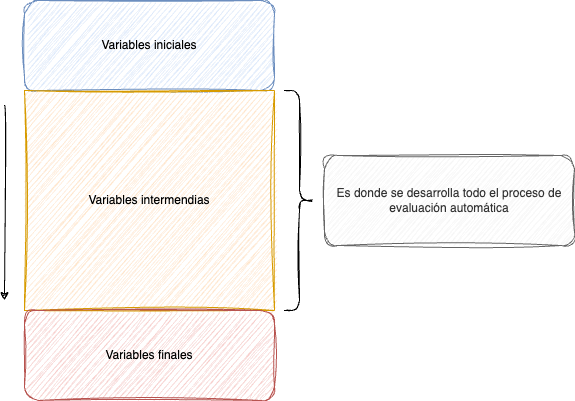
\includegraphics[width=0.7\linewidth]{Graphics/Tape}
	\caption{ Estructura básica de la cinta.}
	\label{fig:Tape}
\end{figure}

Para utilizar esta cinta en un problema como los problemas de enrutamiento de vehículos se debe definir, en primer lugar, las operaciones básicas (o reglas) que aparecerán en cada uno de los problemas. Como se presentan en el capítulo \ref{chapter: VRP}, sección \ref{3-Criterias}, se deben definir los criterios de vecindad que modificarán la solución. 

Estas operaciones se pueden usar en la cinta como ocurre con la Diferenciación automática. La modificación de cada operación se propaga solamente por las ramas que se afectan en cada variante del problema y no se afecta el sistema completo, sino solo ese subproblema, que se debe reevaluar. 

La relación entre las operaciones que se presentan en una función a la que se le aplicará la Diferenciación Automática y las operaciones que componen los criterios de vecindad permite que se utiliza la idea de esta cinta en ambos casos. Al aplicar el criterio de vecindad se obtiene una solución "derivada" de la solución inicial y las operaciones que la componen, al igual que en AD, quedan en la cinta para evaluar solo la parte modificada de la solución.

En este capítulo se presentó el procedimiento de diferenciación automática que utiliza además de un grafo de evaluación, una cinta automática para obtener la derivada de una función matemática.

En el siguiente capítulo se desarrolla esta idea de la diferenciación automática en la evaluación de soluciones vecinas de cualquier VRP.

% Chapter 3 Mezcla y código en Lisp

% Chapter 4 Resultados

% Conclusiones, recomendaciones y bibliografía





























\chapter{Desarrollo de la Evaluación Automática}\label{chapter: Automatic-Eval}

En este capítulo se presenta el desarrollo de los métodos que se ejecutan en la evaluación automática, y la incorporación de la cinta computacional al grafo de evaluación. 

En la sección \ref{3:VRP-eval} se presentan los diferentes problemas de enrutamiento de vehículos que se pueden presentar para evaluar. En la sección \ref{3:init-Solution} se presenta cómo se realiza la evaluación de la solución inicial. En la sección \ref{3:neighbor-solutions} se presenta cómo se modifica este grafo y cómo se realiza la evaluación eficiente de las soluciones vecinas del VRP. En la sección \ref{3:VRP-limits} se presentan algunas variantes que no pueden aplicar la evaluación automática solamente con el grafo de evaluación. En la sección \ref{3:tape-development} se presenta la incorporación de la cinta al grafo de evaluación.

\section{Tipos de VRP a evaluar}\label{3:VRP-eval}
En esta sección se presentan los diferentes tipos de variantes de VRP que pueden presentarse en cualquier escenario.

Existen muchas variantes de VRP y es difícil garantizar que para cualquiera de ellos solo una parte de ese problema se afectará al aplicarle un criterio. Existen tres posibilidades para la evaluación automática de un sistema de enrutamiento de vehículos.

\bf{Definición 1:} \it Llamaremos VRP con clientes independientes a aquellos problemas donde las variables de evaluación o restricción de un cliente (ya sea tiempo, combustible, dinero, distancia, capacidad, etc) no afectan a otro cliente. En ese caso, los clientes son independientes. 

\rm{Este tipo de problemas tiene características especiales en el grafo de evaluación. Cada nodo auxiliar provee directamente al sumador parcial de la ruta y no a otro nodo auxiliar. Se puede notar en la figura \ref{fig:ICVRP}.}

\begin{figure}[htb]
	\centering
	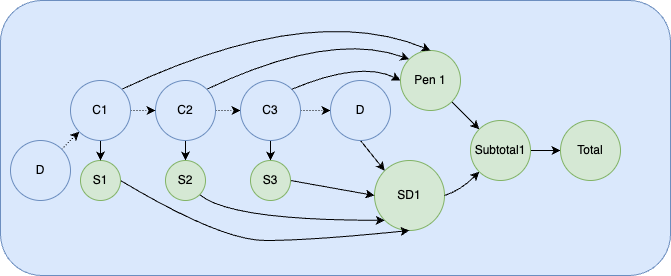
\includegraphics[width=0.7\linewidth]{Graphics/ICVRP}
	\caption{Grafo de evaluación de un VRP con variables independientes.} 
	\label{fig:ICVRP}
\end{figure}

Sobre ese tipo de problemas se tiene el siguiente teorema:
\\\\
\bf{Teorema 1:} \it{En un VRP con clientes independientes, al transformarse un cliente en una ruta solo será necesario reevaluar ese cliente que tributará a la variable de penalización y de suma parcial de la ruta y a la variable del valor final.} 
\\\\
\rm No será necesario reevaluar ningún otro cliente. Al ser independiente del resto no afectará en nada un cambio en su evaluación. Si se agrega o se elimina un cliente, por ejemplo, la evaluación de cada cliente será exactamente igual, no se necesita computar nuevamente la ruta completa. Lo mismo ocurre con rutas disjuntas a la modificada.
\\\\
\bf{Definición 2:} \it Llamaremos VRP con rutas disjuntas a los problemas donde las rutas son independientes. Es decir, las características de los clientes de una ruta no interfieren o modifican a las de la otra ruta.

\rm{Este tipo de problemas es el más común. La mayoría de los VRP se pueden modificar y convertir a este tipo de problemas. La figura \ref{fig:vrp-changeClient} muestra un grafo de evaluación de este tipo.}

\bf{Teorema 2:} \it En los VRP con rutas disjuntas, al ser modificada una de sus rutas será necesario reevaluar, solamente, la ruta modificada, la evaluación de las rutas restantes será la misma después de la modificación del sistema.

\rm Como las demás rutas no se ven afectadas, entonces, por definición, no será necesario comprobar un cambio en su evaluación anterior, el valor y los componentes seguirán siendo los mismos luego que se modifique dicha ruta.

En estos problemas hay dos casos posibles. En primer lugar, la modificación de un cliente afecta la ruta a partir de él hasta cierto cliente o hasta el final de la ruta, es decir, afecta una subruta. Se muestra este caso en la figura \ref{fig:Subway} donde se afecta desde el cliente 1 hasta el cliente 3, sin embargo, no es necesario volver a evaluar el cliente 4, ya que no se ve afectado.

\begin{figure}[htb]
	\centering
	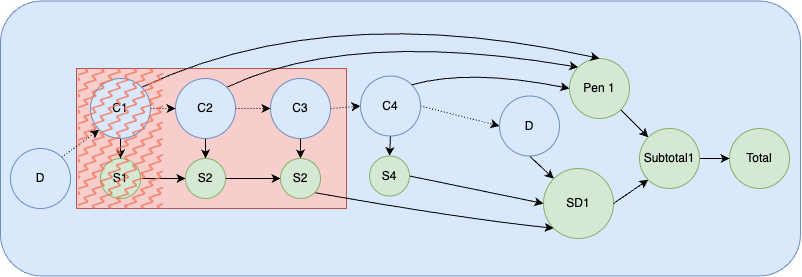
\includegraphics[width=0.7\linewidth]{Graphics/Subway}
	\caption{Grafo de evaluación de un VRP con rutas disjuntas. Caso donde solo se afecta una subruta.} 
	\label{fig:Subway}
\end{figure}


El segundo caso ocurre cuando la modificación de un cliente afecta a toda la ruta, y es necesario reevaluarla completa. Por ejemplo cuando cambia el depósito inicial, o las características de un cliente afectan al cliente anterior. En este caso, se debe reevaluar la ruta completa ya que se afectan todos los clientes. Se muestra este caso en la figura \ref{fig:vrp-changeClient} donde se afecta desde el cliente 1 hasta el cliente 4.

Los VRP con clientes independientes son un subconjunto del primer caso. Y estos, a su vez, son un subconjunto del segundo caso.

\bf{Definición 3:} \it Llamaremos VRP con rutas mezcladas a los problemas donde las rutas no son todas independientes. 

\rm En este caso al trasformarse una ruta que no es disjunta se debe reevaluar todo el sistema teniendo un costo igual a la primera evaluación. 

\section{Evaluación de la solución inicial}\label{3:init-Solution}
En el capítulo \ref{chapter: VRP} se mostró cómo se obtenía el grafo de evaluación a partir de la solución inicial. En esta sección se describe cómo se alcanza la evaluación de esa solución inicial.

En cada nodo principal del grafo de evaluación que representa una entidad del problema se puede acceder a la  información del problema que es relevante a esa entidad \cite{JJ}. Es decir, cada nodo que represente a algún cliente contiene la distancia hacia los demás clientes, las demandas y otra información que sea importante para el cliente. Lo mismo ocurre con el resto de los nodos principales.

A los nodos intermedios creados en el proceso de evaluación se le asocia la operación a realizar sobre las demandas de los clientes y dos métodos, uno para evaluar, y otro para desevaluar, que deshace la evaluación. 

Por ejemplo, si la operación es incrementar la demanda de la ruta, entonces el método evaluar del nodo intermedio asociado a cada cliente suma la demanda del cliente y el valor obtenido del nodo intermedio anterior. El método desevaluar se utiliza para cancelar el método de evaluación de un nodo intermedio.

Al final de cada ruta, el nodo intermedio asociado al último cliente contiene el valor de la evaluación de toda la ruta.

Además de esos nodos intermedios, se crea un nodo penaliza que guarde en cuánto se incumple la demanda de cada cliente en la solución evaluada. En otro nodo intermedio se guarda la evaluación de la ruta una vez penalizada. El valor final de la evaluación de la solución se obtiene a partir de las evaluaciones penalizadas de cada ruta.

Una vez obtenida la evaluación de la solución inicial queda construido totalmente el grafo de evaluación que permitirá evaluar automáticamente soluciones vecinas. Esto se muestra en la siguiente sección.

\section{Obtención y evaluación de las soluciones vecinas} \label{3:neighbor-solutions}

Si se realizan transformaciones a la solución inicial pueden obtenerse soluciones vecinas que se evalúan automáticamente utilizando el grafo de evaluación. En esta sección se presenta cómo se evalúan estas soluciones y una propuesta para que funcione en cualquier VRP.

En el capítulo \ref{chapter: VRP} se mostró cómo se modifica el grafo de evaluación al aplicar una operación sobre la solución inicial. Cada operación es un método que transforma el grafo de evaluación y evalúa o desevalúa los nodos intermedios afectados por la modificación.

Por ejemplo, en la figura \ref{fig:vrp-deleteClient} se aplica la transformación \textbf{eliminar cliente}. Este es un método que recibe las coordenadas del cliente, es decir, el índice de la ruta en la que se encuentra y su posición en la ruta. El nodo intermedio asociado a ese cliente se desevalúa y se elimina, se conecta el nodo intermedio anterior a él con el nodo intermedio siguiente y se evalúan los nodos intermedios afectados. En el ejemplo de la figura, se deben evaluar todos los nodos intermedios siguientes al nodo eliminado.

En \cite{JJ} el autor propone almacenar el nodo extraido en una lista de clientes extraidos.

Los métodos que realizan las operaciones de modificación de una solución son comunes para cualquier VRP que se desee resolver, debido a que los métodos de evaluación y desevaluación reciben la operación a partir del nodo intermedio y, las demandas, a partir de los clientes. 

Un criterio de vecindad es un conjunto de operaciones que modifican la solución inicial, como se plantea en el Capítulo \ref{chapter: VRP}. Al aplicar los métodos de cada una de las operaciones que componen el criterio de vecindad que se utilice, se obtiene la evaluación de la nueva solución. Solamente se reevalúan los nodos del grafo que se modificaron por la aplicación de dichas operaciones. Esta evaluación automática se realiza sin repetir cálculo innecesario.

Este proceso de evaluación automática, como se ha presentado hasta aquí, no funciona para todas las variantes de VRP. En la siguiente sección se presentan algunas de estas variantes.

\section{Limitaciones de algunos VRP}\label{3:VRP-limits}

En esta sección se presentan algunas variantes que no pueden utilizar solamente el grafo de evaluación en la evaluación de sus soluciones vecinas.

En algunos problemas de enrutamiento de vehículos como, por ejemplo, el Problema de Enrutamiento de Vehículos con Entregas y Recogidas Simultáneas o el Problema de Enrutamiento de Vehículos con Ventanas de Tiempo, es necesario evaluar otros nodos del grafo de evaluación que no fueron modificados en la aplicación del criterio de vecindad.

En el Problema de Enrutamiento de Vehículos con Entregas y Recogidas Simultáneas, cada cliente recibe y devuelve una cierta cantidad de producto al mismo tiempo. En esta variante, cada cliente es visitado una única vez, lo que da nombre a este VRP. Esto puede llevar a la violación de la restricción de capacidad, ya que la cantidad total de producto que mantiene el vehículo en cada entrega y recogida puede exceder su capacidad, debido a la recogida de productos mientras se atiende a un cliente durante el recorrido. Por tanto, es necesario penalizar el exceso de carga al visitar cada cliente de la ruta, durante el recorrido y no al final de este.

Si el proceso de penalización se realizara al final de ruta, como ocurre en CVRP (VRP con restricción de capacidad), se puede transformar la solución y reevaluarse hasta el final sin problemas. Sin embargo, si ocurre como en el caso anterior, que la penalización ocurre durante el recorrido, al realizar una modificación de la solución debe verificarse si el cliente modificado participó o no en la penalización de la ruta.

Lo mismo ocurre en el Problema de Enrutamiento de Vehículos con Ventanas de Tiempo, en el que cada cliente tiene un rango de tiempo para satisfacer su demanda. La penalización ocurre cuando el vehículo no llega en ese rango de tiempo que el cliente presenta. Como esta penalización ocurre durante el recorrido y no al final de la ruta, se debe poder verificar en la modificación de la solución, si el cliente afectó o no la variable penalizar.

En la siguiente sección se muestra la propuesta de solución a esta limitante.

\section{Cinta computacional}\label{3:tape-development}

En esta sección se plantean la propuesta de solución que resuelve las limitaciones de algunos VRP frente a la evaluación automática.

El problema que se presenta se basa en la modificación de las variables que se utilizan en la evaluación final del recorrido o ruta. Tal es el caso de la penalización.

Para resolver el problema, se propone implementar la cinta que utiliza la diferenciación automática, que se desarrolla en el capítulo \ref{chapter: AD}. Esta cinta regula las operaciones de modificación sobre la solución inicial. 

En primer lugar, se debe definir cada operación que forma parte de los criterios de vecindad que se aplican a la solución para obtener soluciones vecinas. Al obtener las operaciones y la posición donde se aplicará, se devuelve la parte de la solución que se afecta por esa modificación.

\begin{figure}[htb]
	\centering
	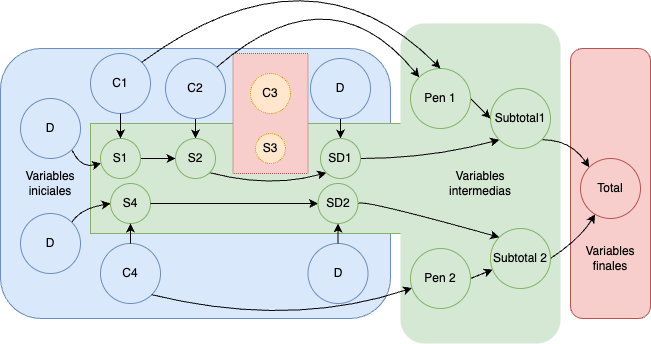
\includegraphics[width=0.7\linewidth]{Graphics/DeleteClient}
	\caption{Grafo de evaluación transformado al eliminar el cliente 3.}
	\label{fig:lisp-deleteClient}
\end{figure}

Si se toma el ejemplo representado en la figura \ref{fig:lisp-deleteClient}, donde se elimina al cliente 3 de la ruta 1 la operación es \textit{eliminar cliente}. A ese método se le pasan los argumentos \textit{ruta: 1} y \textit{posición: 3}. 

A partir de la operación eliminar cliente en la cinta, se verifica la parte de la solución que se modifica y se debe reevaluar. En el caso del ejemplo, se debe reevaluar a partir del cliente anterior hasta el final de la ruta. Para saber si el cliente eliminado afectó la variable penalización este nodo debe ser diferente a los demás nodos intermedios, guardando el valor de penalización de todos los clientes a los que no se les satisfizo la demanda y, por tanto, aumentaron la penalización de la ruta. Por tanto, cuando se elimine al cliente \textit{$C_{3}$} se reevaluará desde el nodo intermedio asociado al nodo del cliente 2 hasta el nodo de salida final, teniendo en cuenta que del nodo penalización se eliminará cualquier penalidad asociada al cliente eliminado.

En el caso de la figura \ref{fig:lisp-insertClient}, donde se inserta el cliente eliminado en la ruta 2, se realiza el mismo proceso de la ruta 1 en la ruta 2. 

\begin{figure}[htb]
	\centering
	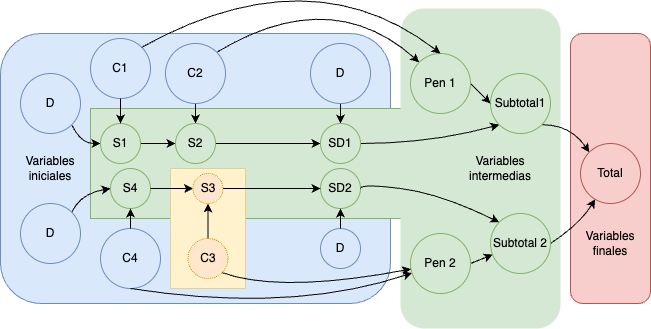
\includegraphics[width=0.7\linewidth]{Graphics/ChangeClient}
	\caption{Grafo de evaluación transformado al eliminar el cliente 3.}
	\label{fig:lisp-insertClient}
\end{figure}

Como la operación es de insertar, entonces, además de evaluar a partir de él, se debe actualizar la variable penalización, en caso de que no se cumpla con la demanda del cliente insertado.

Todas las variables que se modifican en el recorrido en cualquier VRP deben guardar todos los clientes que modifican su valor, como \textbf{penalización} en este caso. Esto hace menos eficiente el algoritmo de evaluación de la solución. En cada variable de ese tipo debe evaluarse el valor de la variable al final de la ruta.

La cinta de evaluación para el ejemplo de la figura \ref{fig:lisp-deleteClient} quedaría de la siguiente manera:

\begin{itemize}
    \item Eliminar cliente (1,3)
    \item Reevaluar (1, 2)
\end{itemize}

Los parámetros de Eliminar cliente son la ruta y la posición del cliente en la ruta. Los parámetros de reevaluar son la ruta y la posición desde donde se debe evaluar.

La cinta de evaluación para el ejemplo de la figura \ref{fig:lisp-insertClient} quedaría de la siguiente manera:

\begin{itemize}
    \item Insertar cliente (2,2)
    \item Reevaluar (2,1)
\end{itemize}

Una solución alternativa es evaluar toda la ruta cuando esta contenga alguna variable que se modifica en el recorrido, como \textbf{penalización}. El cliente que modifique alguna variable durante el recorrido de la ruta debe guardarse en la cinta para verificarse en caso de una modificación para encontrar soluciones vecinas.

La cinta de evaluación para el ejemplo de la figura \ref{fig:lisp-deleteClient} con esta propuesta se muestra en la figura \ref{tape-delete-client}

\begin{figure}[h!]
    \begin{verbatim} 
    clientes_penalizados 
    Eliminar cliente (1,3)
    por cada cliente_i en clientes_penalizados:
             si cliente_i en ruta 1 y posición cliente_i <
                                            posición cliente 3
                Evaluar ruta 1
                terminar
    Reevaluar (1,3)
    \end{verbatim}
    \caption{Cinta de evaluación para el ejemplo \ref{fig:lisp-deleteClient}.\label{tape-delete-client}}
  \end{figure}


La cinta de evaluación para el ejemplo de la figura \ref{fig:lisp-insertClient} se muestra en la figura \ref{tape-insert-client}:

\begin{figure}[h!]
    \begin{verbatim} 
    cliente_i
    Insertar cliente (2,2)
    por cada cliente_i en clientes_penalizados:
             si cliente_i en ruta 2 y posición cliente_i <
                                            posición cliente 2
                Evaluar ruta 2
                terminar
    Reevaluar (2,2)
\end{verbatim}
\caption{Cinta de evaluación para el ejemplo \ref{fig:lisp-insertClient}.\label{tape-insert-client}}
\end{figure}

Al utilizar un criterio de vecindad, varias operaciones se desarrollan en la cinta de evaluación. En la figura \ref{tape-move-client} se muestra el criterio \textit{cambiar un cliente de posición}.

\begin{figure}[h!]
    \begin{verbatim} 
    clientes_penalizados 
    Eliminar cliente (1,3)
    por cada cliente_i en clientes_penalizados:
             si cliente_i en ruta 1 y posición cliente_i <
                                            posición cliente 3
                                                        
                Evaluar ruta 1
                terminar
    Reevaluar (1,3)
    Insertar cliente (2,2)
    por cada cliente_i en clientes_penalizados:
             si cliente_i en ruta 2 y posición cliente_i < 
                                           posición cliente 2
                Evaluar ruta 2
                terminar
    Reevaluar (2,2)
    \end{verbatim}
    \caption{Cinta de evaluación usando el criterio \textit{cambiar un cliente de posición}.\label{tape-move-client}}
  \end{figure}

Esta propuesta realiza más cálculos que las modificaciones que se realizan en la ruta. Pero garantiza que se evalúen los vecinos de cualquier problema de enrutamiento de vehículos. 

En este capítulo se explicaron los métodos que se ejecutan en la evaluación automática de las soluciones vecinas, y la incorporación de una cinta computacional al grafo de evaluación para que sea posible usar esta estrategia en cualquier problema de enrutamiento de vehículos. En el siguiente capítulo se explica cómo se utiliza la evaluación automática en algunas variantes en las que no era posible utilizarse.

% Chapter 4 Resultados

% Conclusiones, recomendaciones y bibliografía




























\chapter{Resultados}\label{chapter: Results}
%Experimentación 

En este capítulo se presentan variantes de problemas de enrutamiento de vehículos a los que no era posible aplicarle la evaluación automática sin realizar modificaciones en el código. Se presentan los cambios necesarios para aplicar la evaluación automática a estos problemas.

Este capítulo se divide en 3 secciones. La sección \ref{4:VRPSPD} presenta la evaluación de vecinos del Problema de Enrutamiento de Vehículos con Recogidas y Entregas. La sección \ref{4:VRPTW} presenta la evaluación de vecinos del Problema de Enrutamiento de Vehículos con Ventanas de Tiempo. La sección \ref{4:Ext} presenta la extensibilidad de este trabajo.

\section{VRP con Recogidas y Entregas simultáneas}\label{4:VRPSPD}
En esta sección se aplica la evaluación automática a un problema de enrutamiento de vehículos con Recogidas y Entregas simultáneas (VRPSPD). Este problema se explica en el capítulo \ref{chapter: Automatic-Eval}, en la sección \ref{3:VRP-limits}.

La figura \ref{fig:VRPSPD-init} muestra una solución inicial de un VRPSPD. Este ejemplo presenta dos rutas, con vehículos de capacidad 20 y 15 respectivamente. El primer vehículo sale del depósito con 5 productos y vista los clientes 1, 2 y 3. El segundo vehículo sale del depósito sin productos y visita los clientes 4 y 5. Cada cliente entrega y recibe un cantidad de productos una vez que es visitado. La cantidad que entrega y que recibe se observa en el nodo que representa a cada cliente.

\begin{figure}[htb]
	\centering
	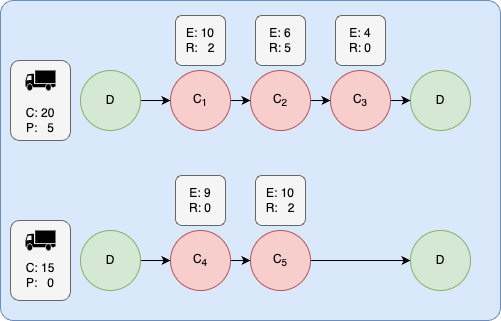
\includegraphics[width=0.5\linewidth]{Graphics/VRPSPD}
	\caption{ Solución inicial del VRPSPD.}
	\label{fig:VRPSPD-init}
\end{figure}

Se deben satisfacer las demandas de cada cliente y obtener la menor distancia para las rutas. El pseudocódigo de la evaluación de la solución inicial se presenta en la figura \ref{vrpspd-sol-code}.

\begin{figure}[h!]
    \begin{verbatim} 
  1  evalúa(S):
  2    new_var distancia_total = 0
  3    para toda ruta r de S:         
  4        new_var demanda_ruta = 0
           new_var penalización = 0
  5        new_var cliente_previo = deposito(r)
  6        para todo cliente c en r:
  7            incrementa distancia_total con...
                          d(cliente_previo, c)
  8            incrementa demanda_ruta con demandas de c 
  9            si demanda_ruta > capacidad del vehículo...
                                 de la ruta r:
  10                penalizar_en_cinta(c)
                    incrementar penalización( 
                        demanda_ruta - capacidad...
                        del vehículo de la ruta r)
  11           cliente_previo = c
  12       incrementa distancia_total con...
                d(c, depósito) 
  13       incrementa distancia_total con penalización
  14    devuelve distancia_total        
  \end{verbatim}
    \caption{Código de evaluación de una solución de un VRPSPD. La operación \texttt{d(x,y)} representa la distancia entre \texttt{x} e \texttt{y}.\label{vrpspd-sol-code}}
\end{figure}

Las demandas del cliente en este problema son los productos que entrega el cliente menos los productos que recoge.

La función $penalizar\_en\_cinta$ guarda el cliente c en la cinta automática en caso de que la demanda de la ruta exceda la capacidad del vehículo en el momento en que se visita al cliente c. Al aplicar los criterios de vecindad en la solución se debe comprobar en la cinta los clientes que penalizaron las rutas antes de evaluar la nueva solución.

 \section{VRP con Ventanas de Tiempo}\label{4:VRPTW}
 En esta sección se aplica la evaluación automática a un problema de enrutamiento de vehículos con Ventanas de Tiempo (VRPTW). Este problema se explica en el capítulo \ref{chapter: Automatic-Eval}, en la sección \ref{3:VRP-limits}.
 
 La figura \ref{fig:VRPSPD-init} muestra una solución inicial de un VRPTW. Este ejemplo, igual que el anterior presenta dos ruta. Cada cliente tiene una hora mínima y una hora máxima entre las que puede ser recogido. Si el vehículo no llega entre esas horas significaría una penalización en la ruta.
 
 \begin{figure}[htb]
     \centering
     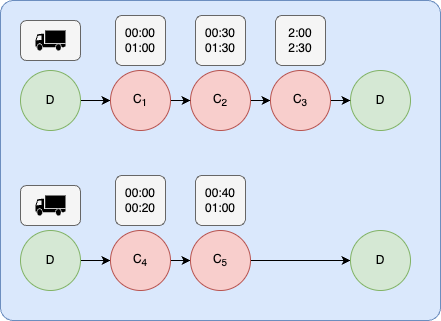
\includegraphics[width=0.5\linewidth]{Graphics/VRPTW}
     \caption{ Solución inicial del VRPTW.}
     \label{fig:VRPSPD-init}
 \end{figure}
 
El pseudocódigo de la evaluación de la solución inicial se presenta en la figura \ref{vrptw-sol-code}.
 
 \begin{figure}[h!]
     \begin{verbatim} 
   1  evalúa(S):
   2    new_var distancia_total = 0
   3    para toda ruta r de S:         
   4        new_var tiempo_ruta = 0
            new_var penalización = 0
   5        new_var cliente_previo = deposito(r)
   6        para todo cliente c en r:
   7            incrementa distancia_total con...
                           d(cliente_previo, c) 
                incrementa tiempo_ruta con...
                           t(cliente_previo, c)
   9            si tiempo_ruta < tiempo mínimo de c
   10                penalizar_en_cinta(c)
                     incrementa penalización con...
                        tiempo_ruta - tiempo mínimo de c
                si tiempo_ruta > tiempo máximo de c
   11                penalizar_en_cinta(c)
                     incrementa penalización con...
                        tiempo máximo de c - tiempo_ruta

   12           cliente_previo = c
   13       incrementa distancia_total con...
                 d(c, depósito)
            incrementa tiempo_ruta con...
                 t(c, depósito) 
   14       incrementa distancia_total con penalización
   15    devuelve distancia_total        
   \end{verbatim}
     \caption{Código de evaluación de una solución de un VRPTW. La operación \texttt{d(x,y)} representa la distancia entre \texttt{x} e \texttt{y}. La operación \texttt{t(x,y)} representa el tiempo del recorrido entre \texttt{x} e \texttt{y}\label{vrptw-sol-code}}
 \end{figure}

La cinta de evaluación automática guarda los clientes que no fueron recogidos en los tiempos asignados. Al aplicar los diferentes criterios de vecindad para modificar la solución y encontrar vecinos se tienen en cuenta las penalizaciones de los clientes para evaluar toda la ruta o a partir del cliente que se modifica. De esta manera se pueden encontrar soluciones vecinas y evaluarse de manera automática, no solo en estos problemas sino en cualquier VRP, que es el objetivo de este trabajo.

En la siguiente sección se presenta cómo extender la propuesta a otros problemas de enrutamiento de vehículos.

\section{Extensibilidad}\label{4:Ext}

En esta sección se comentan algunos problemas diferentes a los presentados en la sección anterior y que se le puede aplicar la evaluación automática.

Para cada variante de VRP deben implementarse diferentes operaciones, no solo mover clientes. Por ejemplo, en el Problema de Enrutamiento de Vehículos con Múltiples Depósitos (MDVRP) se tiene una lista de depósitos y las rutas pueden iniciar y terminar en depósitos distintos. Por ese motivo es necesario implementar las operaciones cambiar el primer depósito de una ruta y cambiar el último depósito de una ruta. Estas operaciones pueden realizarse de la misma manera que las inserciones y extracciones de clientes y el nuevo depósito a insertar se toma de la lista de depósitos disponibles.

Las operaciones implementadas se usan en la cinta computacional para evaluar las soluciones vecinas de la misma manera que se expuso en este capítulo.

A continuación se presentan las conclusiones y recomendaciones del presente trabajo.
% Conclusiones, recomendaciones y bibliografía































%\backmatter
\chapter*{Conclusiones}\label{chapter:Conclusions}
\addcontentsline{toc}{chapter}{Conclusiones}

En este estudio, se ha descrito el proceso de evaluación automática de soluciones vecinas en un Problema de Enrutamiento de Vehículos utilizando un grafo de evaluación. Este enfoque permite evaluar eficientemente las soluciones vecinas sin la necesidad de escribir código específico para esta tarea. 

A partir de este grafo, es posible obtener el valor de cualquier solución vecina al evaluarla en la función objetivo. Se ha resuelto una limitación de la evaluación automática, la cual impedía su aplicación en problemas que involucren penalizaciones durante el recorrido de una ruta.

Se agregó la cinta computacional que extiende este proceso a cualquier problema de enrutamiento de vehículos. Esta estructura permite conocer la parte de la solución afectada al aplicarle a la solución inicial un criterio de vecindad.

Por último, se ha descrito cómo el método de evaluación automática puede ser extendido a otras variantes del Problema de Enrutamiento de Vehículos, utilizando nuevos criterios de vecindad aplicables a cada una de ellas.
\chapter*{Recomendaciones}\label{chapter:Recomendations}
\addcontentsline{toc}{chapter}{Recomendaciones}


Como recomendaciones y trabajos futuros se propone implementar la evaluación automática de soluciones vecinas para variantes de VRP con rutas mezcladas donde no solo sea necesario reevaluar la ruta en la solución vecina, sino todo el sistema. Se propone implementar otras variantes como el Problema de Enrutamiento de Vehículos con Trasbordo y resolverlas con la propuesta presentada.

Se recomienda comprobar con problemas reales la eficiencia de la propuesta presentada y aplicarla a soluciones ya presentadas anteriormente.

Por último se recomienda incorporar esta extensión del Grafo de Evaluación al sistema presentado en \cite{Rodrigo}.
\include{BackMatter/Bibliography}
\include{BackMatter/Glossary}

\end{document}  